%%%%%%%%%%%%%%%%%%%%%%%%%%%%%%%%%%%%%%%%%%%%%%%%%%
% Basic setup. Most papers should leave these options alone.
\documentclass[fleqn,usenatbib]{mnras}

% MNRAS is set in Times font. If you don't have this installed (most LaTeX
% installations will be fine) or prefer the old Computer Modern fonts, comment
% out the following line
\usepackage{newtxtext,newtxmath}
% Depending on your LaTeX fonts installation, you might get better results with one of these:
%\usepackage{mathptmx}
%\usepackage{txfonts}

% Use vector fonts, so it zooms properly in on-screen viewing software
% Don't change these lines unless you know what you are doing
\usepackage[T1]{fontenc}

% Allow "Thomas van Noord" and "Simon de Laguarde" and alike to be sorted by "N" and "L" etc. in the bibliography.
% Write the name in the bibliography as "\VAN{Noord}{Van}{van} Noord, Thomas"
\DeclareRobustCommand{\VAN}[3]{#2}
\let\VANthebibliography\thebibliography
\def\thebibliography{\DeclareRobustCommand{\VAN}[3]{##3}\VANthebibliography}


%%%%% AUTHORS - PLACE YOUR OWN PACKAGES HERE %%%%%

% Only include extra packages if you really need them. Avoid using amssymb if newtxmath is enabled, as these packages can cause conflicts. newtxmatch covers the same math symbols while producing a consistent Times New Roman font. Common packages are:
\usepackage{graphicx}	% Including figure files
\usepackage{float}     % For forcing figure placement
\usepackage{amsmath}	% Advanced maths commands
\usepackage{tikz}
\usetikzlibrary{shapes.geometric, arrows}
\tikzstyle{startstop} = [rectangle, rounded corners, minimum width=3cm, minimum height=1cm,text centered, draw=black, fill=white]
\tikzstyle{process} = [rectangle, minimum width=3cm, minimum height=1cm, text centered, draw=black, fill=white]
\tikzstyle{decision} = [diamond, minimum width=3cm, minimum height=1cm, text centered, draw=black, fill=white]
\tikzstyle{arrow} = [thick,->,>=stealth]

%%%%%%%%%%%%%%%%%%%%%%%%%%%%%%%%%%%%%%%%%%%%%%%%%%

%%%%% AUTHORS - PLACE YOUR OWN COMMANDS HERE %%%%%

% Please keep new commands to a minimum, and use \newcommand not \def to avoid
% overwriting existing commands. Example:
%\newcommand{\pcm}{\,cm$^{-2}$}	% per cm-squared

%%%%%%%%%%%%%%%%%%%%%%%%%%%%%%%%%%%%%%%%%%%%%%%%%%

%%%%%%%%%%%%%%%%%%% TITLE PAGE %%%%%%%%%%%%%%%%%%%

\title[Angular Momentum Evolution of M33 and M31]{Modeling Dynamical Friction-based Angular Momentum Evolution}

\author[Joyce]{
Joyce Thomas,$^{1}$\thanks{E-mail: thomasajoyce@arizona.edu}
Besla Gurtina,$^{1}$
Rathore Himansh$^{1}$
\\
% List of institutions
$^{1}$Steward Observatory, University of Arizona
}


\begin{document}
\label{firstpage}
\pagerange{\pageref{firstpage}--\pageref{lastpage}}
\maketitle

% Abstract of the paper
%\begin{abstract}
%abstract here...
%\end{abstract}


\begin{keywords}
Dark Matter Halo, Dynamical Friction, Galaxy, Galaxy Evolution, Satellite Galaxy, Stellar Disk
\end{keywords}

%%%%%%%%%%%%%%%%%%%%%%%%%%%%%%%%%%%%%%%%%%%%%%%%%%

%%%%%%%%%%%%%%%%% BODY OF PAPER %%%%%%%%%%%%%%%%%%

\section{Introduction}  %%%%%%%%%%%%%%%%%%%%%%%%%%%%%%%%%%%%%%%%

\hspace{\parindent} \textbf{Dynamical friction} is a phenomenon resulting from the gravitational scattering of mass particles from a perturber that acts upon a system to induce angular momentum and energy transfer. This is most often present in large structures consisting of many particles like \textbf{galaxies}, massive gravitationally bound systems consisting of stars, dust, and dark matter. This process is prevalent throughout our universe as many galaxies and systems, not just our own, have \textbf{satellite galaxies}, galaxies orbiting a larger host galaxy inducing gravitational effects and influencing dynamical evolution \citep{Binney_Tremaine-2008}. For example, this direct gravitational influence can affect galactic structures such as the orbital dynamics of the \textbf{stellar disk}, the distribution of stars located within the galaxy flattened to a disk through angular momentum conservation. Additionally, this phenomenon can change the distribution of the \textbf{dark matter halo}, a region that extends far from the galaxy containing most of the galaxy's mass as non-baryonic dark matter. As a result of studying the effects of dynamical friction, much can be revealed about a system's evolution, paving the way for more refined simulation environments for galactic interactions and mergers in the future!

\vspace{10pt}

\hspace{\parindent} The study of dynamical friction is crucial to the development of \textbf{galaxy evolution}. Galaxy evolution refers to the change in a galaxy's composition, structure, age, or other fundamental parameters as a result of interaction with other systems in the universe or the passage of time. For example, dynamical friction slows down both the host and satellite galaxies, influencing merge timescales and as a direct result, the mass growth timescales. Additionally, satellites affected by dynamical friction will slow down, possibly being subject to tidal stripping. This changes the morphology of galaxies and causes regions of over-density and under-density of gasses, leading to star formation and quenching. These important dynamical interactions can change the internal kinematics of both the host and satellite galaxies, leading to a variety of interesting evolutionary effects to be investigated!

\vspace{10pt}

\hspace{\parindent} The understanding of dynamical friction is a complicated one, as it's impossible to observe it playing out in real time. Astronomers do have the capability of surveying a variety of galaxies at different stages of stability and mergers, however with each system differing by a variable degree, it may be difficult to quantify. Instead, Astronomers must rely on simulations based on real-life mass estimates and observations, where these complex interactions can be modeled and propagated in time to observe the effects. One such example is how Rimpei's study utilized a dynamic simulation to derive the dynamical friction effects for barred galaxies between the fast and slow limits, developing a result for bars rotating at an arbitrary speed \citep{RimpeiChiba}. Overall, scientists continue to work on developing their understanding of dynamical friction processes through numerical computation under the guise of DM-dominated systems. This means that simulation results must match the morphology of observable real-life interactions. However, with only the bulge and stellar disk stars available in real-life samples, a large component of dark matter-induced effects are left to be inferred or are yet to be known. 

\vspace{10pt}


\hspace{\parindent} Our understanding of dynamical friction is still incomplete, however. Most dynamical friction models that take into account dark matter interactions operate under the assumption of "cold dark matter." This form of dark matter is characterized by weakly interacting massive particles (WIMPS) moving non-relativistically. On the other hand, galactic interactions with "fuzzy dark matter" have not yet grown to a similar complexity as cold dark matter studies. Fuzzy dark matter particles are extremely light and can behave like a quantum wave, changing the way in which dynamical friction acts \citep{Lancaster_2020}. Another fundamental question is how the angular momentum evolves due to a galactic interaction. One experiment even found the existence of dark matter (DM) wakes as a result of dynamical friction, fueled by the changing resonance patterns of the satellite's orbit around its host. In this study, they found a DM wake produced behind the orbit of the Large Magellanic Cloud (LMC) around the Milky Way (MW), changing the angular momentum distribution of particles within this region as a result \citep{Garavito-Camargo_2019}. 


\noindent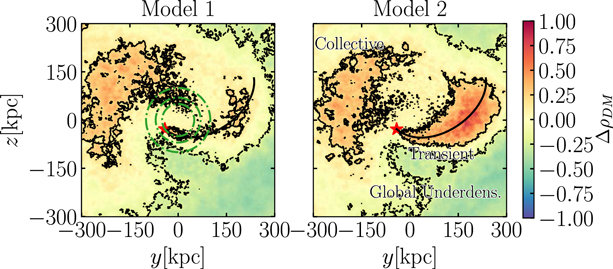
\includegraphics[width=1\linewidth]{DM_wake.jpg}
\noindent\textbf{Figure 1.} Density variations of the Milky Way dark matter distribution resulting from the LMC's passage through the halo. The red star represents the LMC, and the black line: its orbit. The wake is clearly pronounced as an over-density of particles behind it, as shown in red/orange.


\vspace{30pt}
\section{This Project} %%%%%%%%%%%%%%%%%%%%%%%%%%%%%%%%%%%%%%%%

For this investigation, I will analyze how the angular momentum of the M33 and M31 system evolves as a result of dynamical friction interactions. Through analysis of the angular momentum distribution as a function of radius from the center-of-mass point for M31, I will be able to detect the wake caused by M33 and determine its angular momentum change. For the M33 system, I can determine its angular momentum of the entire galaxy with respect to the M31 center of mass frame and see how this system evolves in time as well. Through these metrics, I can see how the angular momentum changes in time with this interaction and model the effects of dynamical friction on the merger. 

\vspace{10pt}

This project addresses the open question proposed by \citep{Garavito-Camargo_2019} in how a dark-matter wake affects the dynamic evolution of the host system. However, in this project, we will be analyzing its effect on the M31-M33 interaction, specifically analyzing the angular momentum evolution. Dynamical friction induces these effects and transfers energy and angular momentum throughout the system; this project will model the dynamical friction implications and not the gravitational dynamics. 

\vspace{10pt}

The dark matter distributions of galaxies can be very large and extend far beyond their stellar disks, meaning that galaxies that get too close will be subject to these forces, changing how galaxies evolve and interact. Due to the presence of dark matter wakes from a satellite body's interaction with the host body's halo, the dynamical timescales can be changed. This means that merging timescales can be accelerated, deformations could occur within the host body, or even a minor merger could evolve into a major merger! Since many large galaxies can have a substantial number of satellite galaxies, it is essential to better model this phenomena to gain a better understanding about how these systems can evolve, refining our simulation accuracy in the process. By taking a deeper look into the angular momentum transfer process, we can gain a better understanding of how dynamical friction can change systems on large timescales. 


\vspace{30pt}
\section{Methodology}  %%%%%%%%%%%%%%%%%%%%%%%%%%%%%%%%%%%%%%%%

Within this study, I will implement the GADGET-3 MW, M31, and M33 merging simulation developed by \cite{vandermarel2012}. This simulation was done as a collisionless N-body model, including stars and dark matter in both a high-resolution and low-resolution capacity. An N-body simulation is one where the system is broken into N interacting particles under the influence of gravity to model an extended system. The initial conditions for this simulation (as modeled by snapshot 0) were determined through observational constraints. The authors constructed the stellar disks by implementing an exponential profile of a specific scale length, and the dark-matter distribution was modeled as a Hernquist profile. 

\vspace{10pt}

To accomplish this study, I will need to determine the dynamical friction effects on angular momentum due to the DM wake-induced transfer. First, we will need to determine the center-of-mass frame for M31 at each time for each particle type for the low-resolution model. Then, for this center-of-mass reference frame, I can update all the position vectors for M31 particles and M33 particles. Next, to further refine the effect of the DM wake, I can implement an angular momentum shell method. Here, I can compute the angular momentum contribution of each particle type in a series of radii from the center of mass position up to a limiting radius. This limiting radius will be a function of scale length and will act to de-bias very far out particles that will dominate the angular momentum contribution, effectively adding random noise. By computing the angular momentum contribution in each shell, the shell containing a majority of the DM wake should see some change as a result of the M33 interaction. Additionally, using the M31 center of mass point, I can determine the angular momentum contribution of the M33 particles and see the M33 system's angular momentum decay as the orbit slows and falls toward the M31 galaxy. Again, there will need to be a limiting radius for M33 as well to counteract the particles very far from the M33 center. Finally, I can continue this in time and see how the system develops, tracking the contribution of the DM wake as a function of time and analyzing how the angular momentum is shifted throughout the system. Figure 2 shows a flowchart outlining my methodology. 

\vspace{10pt}


\scalebox{0.85}{
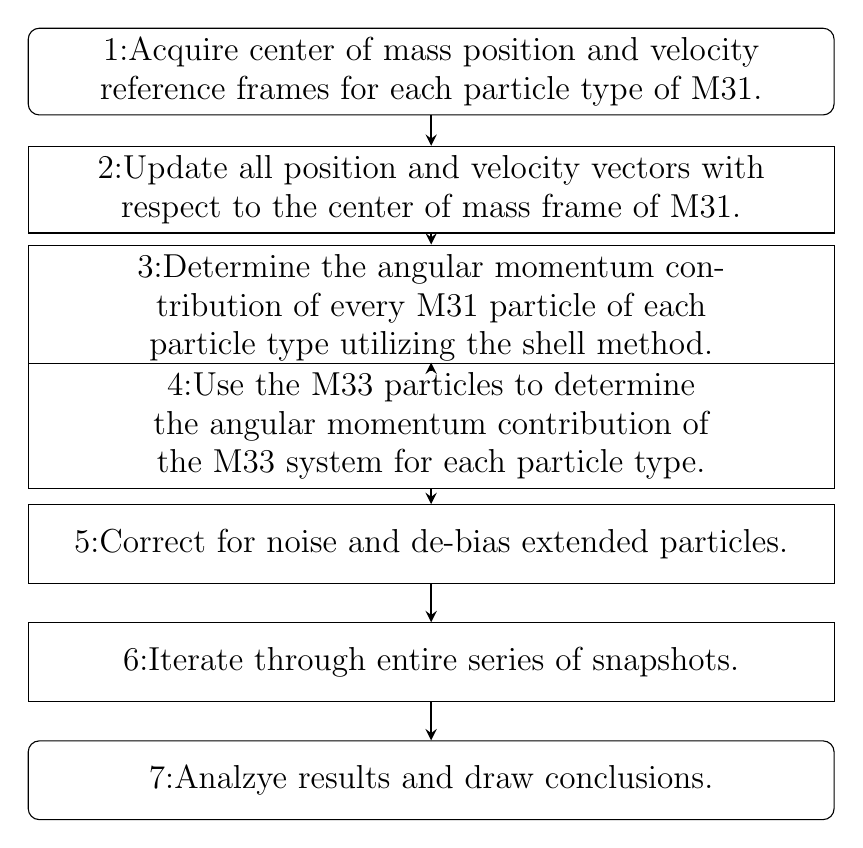
\begin{tikzpicture}[node distance=1.5cm and 0.5cm, every node/.style={text width=10cm, align=center, font=\large}]
        
        \node (start) [startstop] {1:Acquire center of mass position and velocity reference frames for each particle type of M31.};
        \node (step1) [process, below of=start] {2:Update all position and velocity vectors with respect to the center of mass frame of M31.};
        \node (step2) [process, below of=step1] {3:Determine the angular momentum contribution of every M31 particle of each particle type utilizing the shell method.};
        \node (step3) [process, below of=step2] {4:Use the M33 particles to determine the angular momentum contribution of the M33 system for each particle type.};
        \node (step4) [process, below of=step3] {5:Correct for noise and de-bias extended particles.};
        \node (step5) [process, below of=step4] {6:Iterate through entire series of snapshots.};
        \node (end) [startstop, below of=step5] {7:Analzye results and draw conclusions.};

        \draw [arrow] (start) -- (step1);
        \draw [arrow] (step1) -- (step2);
        \draw [arrow] (step2) -- (step3);
        \draw [arrow] (step3) -- (step4);
        \draw [arrow] (step4) -- (step5);
        \draw [arrow] (step5) -- (end);
\end{tikzpicture}
}
\noindent\textbf{Figure 2.} Methodology visualized through flowchart outlining each step of the experiment

\vspace{10pt}

To implement this study, I will develop a code in python to do these calculations. Specifically when taking the displacement vector for the new reference frame the equation for such is outlined as: $ \vec{r_{com_i}} = \vec{r_i}-\vec{R_{com_i}} $, where $ \vec{r_{com_i}} $ is the position vector in the center of mass frame for any "ith" particle, $ \vec{r_i} $ is the position vector for the "ith" particle, and $ \vec{R_{com_i}}$ is the position for the center of mass for M31. The same would apply for the velocity vectors as well. The contribution of angular momentum of a specific particle will be: $ \sum_{i=1}^{N} \vec{L_i} = \sum_{i=1}^{N} m_i (\vec{r_{com_i}} \times \vec{v_{com_i}}) $. The limiting radius for each galaxy would be 3 times the scale length of the Hernquist profile for the dark matter distribution \citep{hernquist1990}.

\vspace{10pt}

The plots generated by this code will be twofold: One plot will be highlighting the orbital decay of the M33 system, and another will highlight the effect of the DM wake on the angular momentum of M31. Each plot will be a representation in time, where time is on the x-axis and angular momentum is on the y-axis. By showing this angular momentum evolution in time, the effects of dynamical friction can be visualized and characterized. 

\vspace{10pt}

Due to the DM wake created by M33's passage through M31's dark matter halo, this will create an overdensity of particles behind M33's trajectory. This will cause a net force backward, making the orbit slower over time. Without this rotational inertia, M33's orbit will decay inward towards M31. Overall, there will be a decrease in the angular momentum of M33, where the transfer will go into the M31 system via the dark matter distribution. The DM wake caused by M33's passage will cause an over-density of particles in that shell, raising the total angular momentum in that region, accepting the transfer from M33. 

\vspace{30pt}
\section{Results}
%%%%%%%%%%%%%%%%%%%%%%%%%%%%%%%%%%%%%%%%

After analyzing the resulting interaction within the simulation, the results outlined in Figure 1 found the presence of an angular momentum overabundance near the radial position of M33. Figure 1 shows an example of one frame of the GIF generated by the program, showing a higher distribution of angular momentum near the location of M33. The entire GIF is available in my GitHub repository linked \href{https://github.com/ThomasaturnV/ASTR400B/blob/main/ResearchAssignments/ResearchAssignment6/M31_AngularMomentumEvolution.gif}{here}. This overabundance of angular momentum implies the presence of a DM wake, generating a higher density of angular momentum at a similar radial position as the satellite galaxy.

\noindent
\includegraphics[width=1\linewidth]{M31_AngularMomentumEvolution-T6.857.png}
\noindent\textbf{Figure 3.} One frame of the angular momentum distribution GIF at a time of 6.857 Gyrs. The total angular momentum (y-axis) calculated within each shell of the radial distribution (x-axis) goes out to 15 scale lengths. The gray dotted line represented the radial position of M33. The entire GIF is available \href{https://github.com/ThomasaturnV/ASTR400B/blob/main/ResearchAssignments/ResearchAssignment6/M31_AngularMomentumEvolution.gif}{here}.

\vspace{10pt}

Due to the creation of this DM wake, angular momentum is being transferred to M31 as M33's orbital angular momentum decreases as a result. This can be seen in Figure 2, as M33's total orbital angular momentum is decreasing from the dynamical friction effects of this galactic interaction. The vertical fluctuations present in the graph are caused by the complicated non-Keplerian orbit of M33 around M31. However, the large dip located around 4 Gyr is likely due to M33 "falling into" M31 as the velocity and position vectors grow nearly parallel. At the end of the simulation, the orbital angular momentum of M33 around M31 has decreased by about a factor of 100 due to dynamical friction!


\noindent
\includegraphics[width=1\linewidth]{M33OrbitalAngMomEvolution.png}
\noindent\textbf{Figure 4.} Shown above is the total orbital angular momentum of M33 (y-axis) around M31 as a function of time (x-axis). M33 was treated as a point mass for the simplicity of the orbital angular momentum calculation. The distribution decays over time due to the effects of dynamical friction.  


\vspace{30pt}
\section{Discussion}
%%%%%%%%%%%%%%%%%%%%%%%%%%%%%%%%%%%%%%%%
The presence of the DM wake detected in Figure 3 provides an explanation as to the angular momentum evolution of the system. Since dynamical friction is causing an over-abundance of DM particles behind M33, this would appear at or near the same radial position as M33, as the shell method would encase portions of this wake within one or more bins. This over-abundance of particles will cause a gravitational attraction, ultimately slowing the movement of M33 or decaying its orbit, influencing its angular momentum evolution. This takes place in the form of an angular momentum transfer between the two systems of M33 and M31, as seen by the decrease detected in Figure 4. This result agrees with the hypothesized scenario proposed at the origin of this study. 

\vspace{10pt}

This result will lead researchers to better quantify the effects of dynamical friction on these evolving systems. For example, the detections of a DM wake within the M33-M31 system seems to imply that a DM wake may be more common than previously thought and the effects seen from the LMC and the Milky Way in \citep{Garavito-Camargo_2019} may not be a peculiar event. Such drastic angular momentum changes can lead to interesting results with galactic mergers. Even a minor merger can lead to a reasonable decrease in orbital angular momentum. Better understanding these effects can lead to a firmer grasp on the barrier between minor and major mergers as a particular interaction could easily transition the boundary between the two with dynamical friction being the catalyst for this. 

\vspace{10pt}

Due to the limitations of this study there are some uncertainties in the results. For example, M33 was approximated as a point mass located at its center of mass point calculated from its DM particles. This may give some orbital angular momentum inconsistencies as M33 is truly an extended body. Additionally, throughout this investigation the only particle type considered were the dark matter particles, as this type of matter vastly dominates the mass budget of each system. However due to this approximation some angular momentum considerations are not fully captured, potentially skewing all the results to a lower value. Another potential limitation could be the resolution of the study, as the simulation used was the low resolution one. This choice was due to hardware limitations in order to ease computational simplicity. However due to this change the finer structure of the DM wake could be lost as a result, instead capturing only the general trend.  




%%%%%%%%%%%%%%%%%%%% REFERENCES %%%%%%%%%%%%%%%%%%

% The best way to enter references is to use BibTeX:

\bibliographystyle{mnras}
\bibliography{Citations} % if your bibtex file is called example.bib


% Altern,atively you could enter them by hand, like this:
% This method is tedious and prone to error if you have lots of references
%\begin{thebibliography}{99}
%\bibitem[\protect\citeauthoryear{Author}{2012}]{Author2012}
%Author A.~N., 2013, Journal of Improbable Astronomy, 1, 1
%\bibitem[\protect\citeauthoryear{Others}{2013}]{Others2013}
%Others S., 2012, Journal of Interesting Stuff, 17, 198
%\end{thebibliography}

%%%%%%%%%%%%%%%%%%%%%%%%%%%%%%%%%%%%%%%%%%%%%%%%%%

%%%%%%%%%%%%%%%%% APPENDICES %%%%%%%%%%%%%%%%%%%%%

%\appendix

%\section{Some extra material}

%If you want to present additional material which would interrupt the flow of the main paper,
%it can be placed in an Appendix which appears after the list of references.

%%%%%%%%%%%%%%%%%%%%%%%%%%%%%%%%%%%%%%%%%%%%%%%%%%


% Don't change these lines
\bsp	% typesetting comment
\label{lastpage}
\end{document}

% End of mnras_template.tex
